\documentclass[11pt,a4paper]{article}

% ============================================================================
% PACKAGES
% ============================================================================
\usepackage[utf8]{inputenc}
\usepackage[T1]{fontenc}
\usepackage{amsmath,amssymb,amsthm}
\usepackage{mathtools}
\usepackage{geometry}
\usepackage{graphicx}
\usepackage{hyperref}
\usepackage{cleveref}
\usepackage{booktabs}
\usepackage{array}
\usepackage{multirow}
\usepackage{xcolor}
\usepackage{tcolorbox}
\usepackage{tikz}
\usepackage{pgfplots}
\usepackage{enumitem}
\usepackage{float}
\usepackage{caption}
\usepackage{subcaption}
\usepackage{fancyhdr}
\usepackage{natbib}

% ============================================================================
% PAGE GEOMETRY
% ============================================================================
\geometry{
    left=2.5cm,
    right=2.5cm,
    top=2.5cm,
    bottom=2.5cm
}

% ============================================================================
% TIKZ LIBRARIES
% ============================================================================
\usetikzlibrary{arrows.meta, positioning, shapes.geometric, calc, decorations.pathmorphing}
\pgfplotsset{compat=1.18}

% ============================================================================
% THEOREM ENVIRONMENTS
% ============================================================================
\theoremstyle{definition}
\newtheorem{definition}{Definition}[section]
\newtheorem{remark}{Remark}[section]
\newtheorem{example}{Example}[section]
\newtheorem{assumption}{Assumption}[section]

\theoremstyle{plain}
\newtheorem{theorem}{Theorem}[section]
\newtheorem{proposition}{Proposition}[section]
\newtheorem{lemma}{Lemma}[section]
\newtheorem{corollary}{Corollary}[section]

% ============================================================================
% CUSTOM BOXES
% ============================================================================
\tcbuselibrary{skins,breakable}

\newtcolorbox{keyinsight}[1][]{
    enhanced,
    breakable,
    colback=blue!5!white,
    colframe=blue!75!black,
    fonttitle=\bfseries,
    title={Key Insight},
    #1
}

\newtcolorbox{implementation}[1][]{
    enhanced,
    breakable,
    colback=green!5!white,
    colframe=green!50!black,
    fonttitle=\bfseries,
    title={Implementation},
    #1
}

% ============================================================================
% CUSTOM COMMANDS
% ============================================================================
\newcommand{\R}{\mathbb{R}}
\newcommand{\E}{\mathbb{E}}
\newcommand{\Var}{\mathrm{Var}}
\newcommand{\sgn}{\mathrm{sgn}}
\newcommand{\clip}{\mathrm{clip}}
\newcommand{\med}{\mathrm{med}}
\newcommand{\MAD}{\mathrm{MAD}}

\renewcommand{\vec}[1]{\boldsymbol{#1}}
\newcommand{\bphi}{\boldsymbol{\phi}}
\newcommand{\btheta}{\boldsymbol{\theta}}

% ============================================================================
% HYPERREF SETUP
% ============================================================================
\hypersetup{
    colorlinks=true,
    linkcolor=blue!70!black,
    citecolor=green!50!black,
    urlcolor=blue!70!black,
    pdftitle={A Mirror-Symmetric AMM for Hyperliquid},
}

% ============================================================================
% HEADER/FOOTER
% ============================================================================
\pagestyle{fancy}
\fancyhf{}
\fancyhead[L]{\small Mirror-Symmetric AMM}
\fancyhead[R]{\small Hyperliquid}
\fancyfoot[C]{\thepage}
\renewcommand{\headrulewidth}{0.4pt}

% ============================================================================
% TITLE
% ============================================================================
\title{
    \textbf{A Mirror-Symmetric AMM for Hyperliquid}\\[0.5em]
    \large Dual Liquidity Descriptions via Order Book--Curve Duality
}

\author{}
\date{\today}

% ============================================================================
% DOCUMENT BEGIN
% ============================================================================
\begin{document}

\maketitle

% ============================================================================
% ABSTRACT
% ============================================================================
\begin{abstract}
\noindent
We present an automated market maker (AMM) for Hyperliquid that treats order books and pricing curves as dual descriptions of liquidity, connected by a structure-preserving map. The design exploits Hyperliquid's dual-venue architecture---HyperEVM smart contracts with synchronous access to HyperCore order book state---to build an AMM whose parameters adapt to real-time microstructure signals.

The core contribution is a \emph{duality-preserving parameterization}: order book observables (depth, imbalance, volatility) map to curve parameters (curvature, spread) via transformations that preserve convexity and no-arbitrage structure. We derive the optimal pricing potential from LP profit maximization under adverse selection, showing that the $\tanh$-regularized quadratic form emerges from inventory boundary constraints. 

The architecture comprises an AMM on HyperEVM with real-time parameter updates and an \emph{instanton allocator} that triggers discrete regime transitions when market conditions justify moving capital between the continuous AMM surface and discrete order book execution. The allocator computes an action signal from inventory, oracle tier, and spread conditions, emitting rebalancing decisions when thresholds are exceeded.

\end{abstract}

\tableofcontents
\newpage

% ============================================================================
% SECTION 1: INTRODUCTION
% ============================================================================
\section{Introduction}
\label{sec:intro}

\subsection{The Problem: Information-Blind AMMs}

Standard automated market makers operate without knowledge of broader market structure. A Uniswap pool prices assets according to its reserve ratio, regardless of whether the surrounding order book shows massive sell pressure, elevated volatility, or thin liquidity. This information asymmetry creates systematic value extraction: informed traders exploit stale AMM prices, imposing adverse selection costs on liquidity providers.

The conventional response---wider spreads, higher fees---sacrifices capital efficiency. A more sophisticated approach would allow the AMM to \emph{see} market microstructure and adapt accordingly.

\subsection{The Opportunity: Hyperliquid's Dual Venues}

Hyperliquid provides a unique infrastructure: HyperEVM smart contracts can synchronously read HyperCore order book state via precompiled contracts. This enables an AMM that observes depth profiles, order flow imbalance, and price volatility \emph{within the same transaction} as a swap. The question becomes: how should this information inform pricing?

\subsection{Our Approach: Duality-Preserving Parameterization}

We propose treating the order book and AMM curve not as separate systems but as \emph{dual descriptions} of the same underlying liquidity structure. This perspective, inspired by duality phenomena in mathematical physics, generates specific design constraints:

\begin{enumerate}
    \item Both descriptions should derive from a common \emph{generating function} (potential)
    \item The map between descriptions must \emph{preserve structure}---specifically, convexity and no-arbitrage conditions
    \item The natural coordinates differ: order books use discrete price levels; AMMs use continuous inventory
    \item Transitions between regimes should occur via \emph{instanton-like jumps} when the action favors discrete over continuous evolution
\end{enumerate}

These constraints are not philosophical---they have algorithmic consequences. The requirement that the parameterization map preserves convexity imposes sign constraints on how order book signals affect curve parameters. The generating function structure ensures path-independent pricing. The instanton mechanism enables capital to switch between AMM and order book modes when conditions warrant.

\subsection{Contributions}

\begin{enumerate}
    \item \textbf{Duality framework}: A precise formulation of order book--curve duality with structure-preserving maps (Section~\ref{sec:philosophy}).
    
    \item \textbf{Optimal potential derivation}: We derive the LP-optimal pricing potential under adverse selection and inventory constraints, showing the $\tanh$-regularized quadratic form is not ad-hoc but emerges from the optimization (Section~\ref{sec:potential}).
    
    \item \textbf{Instanton allocator}: A decision system that computes an action signal and triggers regime transitions between continuous AMM and discrete order book modes (Section~\ref{sec:allocation}).
    
    \item \textbf{Complete implementation}: Deployed smart contracts demonstrating the architecture on a local test environment (Sections~\ref{sec:oracle}--\ref{sec:safety}).
\end{enumerate}

\subsection{Scope and Limitations}

We develop a proof-of-concept architecture deployed on a local Hardhat fork of HyperEVM. The duality framework provides design guidance, not a mathematical theorem; the LP analysis uses stylized models. The implementation demonstrates the core concepts with simplified components (mock oracle, basic yield vault). We are explicit about what is derived versus engineered.


% ============================================================================
% SECTION 2: HYPERLIQUID ARCHITECTURE
% ============================================================================
\section{Hyperliquid Architecture}
\label{sec:hyperliquid}

Hyperliquid combines a high-performance order book execution layer (HyperCore) with EVM-compatible smart contracts (HyperEVM). We summarize the primitives relevant to our design.

\subsection{HyperCore}

The native execution layer provides:
\begin{itemize}
    \item Central limit order books for spot and perpetual markets
    \item Sub-second matching with deterministic execution
    \item Native oracle prices derived from order book state
    \item Position and balance tracking at consensus level
\end{itemize}

\subsection{HyperEVM Integration}

Two system-level primitives enable cross-venue composability:

\paragraph{Read Precompiles.} Contracts at addresses \texttt{0x0...0800+} expose HyperCore state to EVM execution. Critically, reads are \emph{synchronous}: within a transaction, the contract sees HyperCore state consistent with block construction time. This enables atomic validation of order book conditions during swaps.

\paragraph{CoreWriter.} The system contract at \texttt{0x333...333} allows EVM contracts to emit logs interpreted as HyperCore actions (order placement, cancellation, transfers).

\subsection{API Wallets}

Off-chain signing keys authorized to place HyperCore orders on behalf of an EVM address. This enables high-frequency quote management without per-order gas costs, while on-chain contracts maintain control logic.

\begin{figure}[H]
\centering
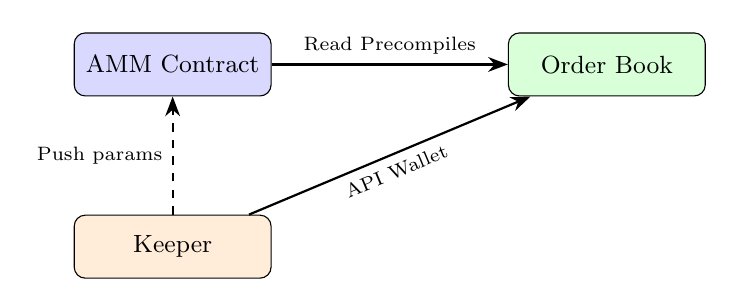
\begin{tikzpicture}[
    node distance=1.2cm and 2.5cm,
    box/.style={rectangle, draw, rounded corners, minimum width=2.5cm, minimum height=0.8cm, align=center, font=\small},
    arrow/.style={-{Stealth[length=2.5mm]}, thick}
]
\node[box, fill=blue!15] (amm) {AMM Contract};
\node[box, fill=green!15, right=3cm of amm] (ob) {Order Book};
\node[box, fill=orange!15, below=1.5cm of amm] (keeper) {Keeper};

\draw[arrow] (amm) -- node[above, font=\scriptsize] {Read Precompiles} (ob);
\draw[arrow, dashed] (keeper) -- node[left, font=\scriptsize] {Push params} (amm);
\draw[arrow] (keeper) -- node[below, sloped, font=\scriptsize] {API Wallet} (ob);
\end{tikzpicture}
\caption{Integration architecture. Solid arrows: synchronous reads. Dashed: asynchronous updates.}
\label{fig:arch}
\end{figure}


% ============================================================================
% SECTION 3: DESIGN PHILOSOPHY
% ============================================================================
\section{Design Philosophy: Order Book--Curve Duality}
\label{sec:philosophy}

\subsection{The Duality Perspective}

Consider two ways to describe liquidity for a trading pair:

\textbf{Order book description}: A collection of price levels $\{p_i\}$ with quantities $\{Q_i\}$, specifying discrete willingness to trade at each price. This is \emph{enumerative}---we count liquidity at each level.

\textbf{Curve description}: A continuous function $P(q)$ specifying marginal price as a function of inventory $q$. This is \emph{geometric}---we describe a smooth surface.

These appear different, but both encode the same economic object: a schedule of prices at which liquidity is available. The insight is that a \emph{principled map} should relate them, and that capital can transition between these representations when economically justified.

\subsection{Structure Preservation}

Not any map will do. We require:

\begin{definition}[Structure-Preserving Map]
A parameterization $\bphi \mapsto \btheta$ from order book observables to curve parameters is \emph{structure-preserving} if:
\begin{enumerate}
    \item \textbf{Convexity preservation}: Higher order book depth maps to lower curve curvature, and vice versa, such that the induced pricing function remains convex.
    \item \textbf{Monotonicity}: The map is monotonic in natural senses---more adverse conditions (higher volatility, lower depth) yield more conservative pricing (higher curvature, wider spreads).
    \item \textbf{No-arbitrage}: The curve remains arbitrage-free under parameter changes.
\end{enumerate}
\end{definition}

These constraints generate the sign conditions in our parameterization map (Section~\ref{sec:map}).

\subsection{The Generating Function}

Both descriptions should derive from a common object. For the AMM, this is the \emph{potential} $F(q)$:
\begin{itemize}
    \item Prices are derivatives: $\log P(q) = F'(q)$
    \item Swap costs are differences: $\text{Cost}(q_0 \to q_1) = F(q_1) - F(q_0)$
    \item Convexity ($F'' > 0$) ensures positive liquidity
\end{itemize}

The order book implicitly defines a potential via cumulative depth. The duality map relates the parameters of these potentials.

\subsection{Instanton Transitions}

In physics, an \emph{instanton} is a non-perturbative solution describing tunneling between classical vacua---a discrete jump when continuous evolution is energetically unfavorable. We borrow this concept:

\begin{definition}[Instanton Regime Transition]
A capital allocation is \emph{instanton-like} if it transitions discretely between AMM (continuous) and order book (discrete) modes when a computed action signal exceeds a threshold, rather than evolving parameters smoothly.
\end{definition}

This is not a claim about quantum field theory---it is a design metaphor. The action signal $S$ aggregates risk factors (inventory imbalance, oracle deviation, spread stress). When $S$ crosses a threshold, the system signals that capital should move from the continuous AMM surface to discrete order book quotes, or vice versa.

\begin{keyinsight}
The duality perspective is not merely philosophical. It generates:
\begin{enumerate}
    \item Sign constraints on the parameterization map
    \item The requirement that prices derive from a potential (ensuring path-independence)
    \item A criterion for which order book statistics are relevant (those affecting the potential's shape)
    \item A decision rule for when to transition between continuous and discrete liquidity modes
\end{enumerate}
\end{keyinsight}

\subsection{What This Is Not}

We do not claim a mathematical theorem relating order books to AMMs. The duality is a \emph{design heuristic} that constrains the space of reasonable architectures. Its value lies in the structure it imposes, not in formal equivalence.


% ============================================================================
% SECTION 4: THE MODEL
% ============================================================================
\section{The Model}
\label{sec:model}

\subsection{State and Notation}
\label{sec:notation}

\begin{definition}[System State]
The AMM maintains:
\begin{align}
    q &\in \R: \text{signed inventory (positive = long base asset)} \\
    \btheta &= (c, \lambda, s): \text{curve parameters} \\
    p_{\mathrm{ref}} &\in \R_{>0}: \text{reference price}
\end{align}
where $c = \log p_{\mathrm{ref}}$ is the log-price center, $\lambda > 0$ is curvature, and $s \geq 0$ is the spread parameter.
\end{definition}

The inventory coordinate $q$ is normalized: $q = 0$ corresponds to balanced reserves, $q > 0$ means the AMM holds excess base asset.

\subsection{Order Book Signals}
\label{sec:signals}

We extract a compressed representation from the order book that captures pricing-relevant information.

\begin{definition}[Order Book Observables]
\label{def:observables}
From a HyperCore order book snapshot, define:
\begin{align}
    p_0 &= \frac{p_{\mathrm{bid}}^{(1)} + p_{\mathrm{ask}}^{(1)}}{2} && \text{(mid price)} \\
    D &= D^+ + D^- && \text{(total depth within band $\pm\delta$)} \\
    I &= \frac{D^+ - D^-}{D^+ + D^-} \in [-1,1] && \text{(imbalance)} \\
    \sigma &= 1.4826 \cdot \med_i |r_i - \med_j r_j| && \text{(robust volatility)}
\end{align}
where $D^\pm$ is quote-currency depth on ask/bid side within $\delta$ of mid (e.g., $\delta = 1\%$), and $\{r_i\}$ are recent log-returns.
\end{definition}

\paragraph{Why these signals?}
\begin{itemize}
    \item \textbf{Mid price $p_0$}: Anchors the curve to market consensus.
    \item \textbf{Depth $D$}: Measures market capacity. Low depth signals fragility requiring conservative pricing.
    \item \textbf{Imbalance $I$}: First-order predictor of informed flow direction. $I > 0$ (ask-heavy) suggests expected price decrease.
    \item \textbf{Volatility $\sigma$}: Regime indicator. High volatility increases inventory risk.
\end{itemize}

\subsection{The Parameterization Map}
\label{sec:map}

The map from observables to curve parameters:

\begin{definition}[Parameterization Map]
\label{def:map}
\begin{align}
    c &= \log p_{\mathrm{ref}} \label{eq:map_c} \\
    \lambda &= \lambda_0 + \alpha_\sigma \sigma + \alpha_I |I| + \alpha_D / D \label{eq:map_lambda} \\
    s &= s_0 + \beta_\sigma \sigma + \beta_I |I| \label{eq:map_s}
\end{align}
with calibration constants $\lambda_0, s_0 > 0$ and $\alpha_\sigma, \alpha_I, \alpha_D, \beta_\sigma, \beta_I \geq 0$.
\end{definition}

\begin{proposition}[Structure Preservation]
\label{prop:structure}
The map satisfies the structure-preservation requirements:
\begin{enumerate}
    \item \textbf{Monotonicity}: $\partial \lambda / \partial \sigma > 0$, $\partial \lambda / \partial |I| > 0$, $\partial \lambda / \partial D < 0$.
    \item \textbf{Convexity}: For $\lambda > 0$, the induced pricing curve is convex.
    \item \textbf{Boundedness}: Given bounded inputs, outputs remain bounded.
\end{enumerate}
\end{proposition}

The signs encode economic logic:
\begin{itemize}
    \item Higher volatility $\Rightarrow$ more curvature (charge more for inventory risk)
    \item Higher imbalance $\Rightarrow$ more curvature (protect against informed flow)
    \item Lower depth $\Rightarrow$ more curvature (market is fragile)
\end{itemize}

\subsection{The Pricing Potential}
\label{sec:potential}

We now derive the optimal form of the pricing potential.

\subsubsection{LP Optimization Problem}

Consider an LP maximizing expected profit under:
\begin{itemize}
    \item Uninformed flow arriving at rate $\mu_U$ with random direction
    \item Informed flow arriving at rate $\mu_I$ knowing future price $p^*$
    \item Inventory bounded: $|q| \leq q_{\max}$
    \item Price impact via potential: $\log P(q) = F'(q)$
\end{itemize}

The LP's value function $V(q)$ satisfies the Hamilton-Jacobi-Bellman equation:
\begin{equation}
    0 = \max_{F} \left[ \mu_U \cdot \E[\text{fee revenue}] - \mu_I \cdot \E[\text{adverse selection loss}] + \frac{\sigma^2}{2} V''(q) \right]
    \label{eq:hjb}
\end{equation}
subject to boundary conditions $V'(\pm q_{\max}) = \mp \infty$ (infinite cost at inventory limits).

\subsubsection{Solution}

\begin{theorem}[Optimal Potential Form]
\label{thm:optimal}
Under the model above, the LP-optimal pricing rule has the form:
\begin{equation}
    \log P(q) = c + \lambda^* q + \eta \tanh(q/\eta)
    \label{eq:optimal_price}
\end{equation}
where $\lambda^* \propto \sigma\sqrt{\mu_I/\mu_U}$ and $\eta \propto q_{\max}$.
\end{theorem}

\begin{proof}[Proof sketch]
The HJB equation~\eqref{eq:hjb} with reflecting boundaries at $\pm q_{\max}$ yields a solution of the form $V(q) = Aq^2 + B\log\cosh(q/\eta) + C$. The optimal pricing rule is $\log P = V'$, giving the stated form. The $\tanh$ term arises from the boundary conditions---without inventory limits, pure quadratic ($\lambda q$) would suffice. Full derivation in Appendix~\ref{app:derivation}.
\end{proof}

\begin{keyinsight}
The $\tanh$ saturation is not an ad-hoc design choice. It emerges from the optimization when inventory is bounded. This provides theoretical grounding for the potential family.
\end{keyinsight}

\subsubsection{The Potential Function}

Integrating~\eqref{eq:optimal_price}:

\begin{definition}[Pricing Potential]
\begin{equation}
    F_\theta(q) = cq + \frac{\lambda}{2}q^2 + \eta \log\cosh(q/\eta)
    \label{eq:potential}
\end{equation}
\end{definition}

Properties:
\begin{itemize}
    \item $F \in C^\infty(\R)$ (smooth)
    \item $F''(q) = \lambda + \eta^{-1}\mathrm{sech}^2(q/\eta) > 0$ (convex)
    \item $F''(q) \in [\lambda, \lambda + \eta^{-1}]$ (bounded curvature)
    \item $F(q) \sim cq + \frac{\lambda}{2}q^2 + |q|$ as $|q| \to \infty$ (linear growth in tails)
\end{itemize}

\subsection{Spread and Fee Construction}
\label{sec:spread}

\begin{definition}[Executable Prices]
\begin{align}
    P_{\mathrm{ask}}(q) &= P(q) \cdot (1 + s) \\
    P_{\mathrm{bid}}(q) &= P(q) \cdot (1 - s)
\end{align}
where $P(q) = \exp(F'(q)) = p_{\mathrm{ref}} \exp(\lambda q + \tanh(q/\eta))$.
\end{definition}

The spread $s$ covers:
\begin{itemize}
    \item Execution costs (gas, slippage in hedging)
    \item LP compensation for providing liquidity
    \item Risk premium scaling with volatility and imbalance
\end{itemize}

In the implementation, spread is tiered based on oracle deviation (Section~\ref{sec:oracle}).

\subsection{Swap Execution}
\label{sec:swap}

A trader exchanging $\Delta X$ of base asset:

\begin{enumerate}
    \item \textbf{Read state}: Current inventory $q_0$, parameters $\btheta$, live oracle $p_{\mathrm{live}}$.
    
    \item \textbf{Validate oracle}: Check deviation tier. Adjust spread based on tier (Section~\ref{sec:oracle}).
    
    \item \textbf{Compute output}: 
    \begin{align}
        q_1 &= q_0 \pm \Delta X \\
        \text{quote cost} &= \text{midPrice}(q_{\text{mid}}) \cdot \text{baseDelta} \cdot (1 \pm s_{\text{eff}})
    \end{align}
    where $q_{\text{mid}} = (q_0 + q_1)/2$ and $s_{\text{eff}}$ depends on oracle tier.
    
    \item \textbf{Check inventory cap}: Verify $|q_1| \leq q_{\max}$.
    
    \item \textbf{Execute}: Transfer assets, update $q \leftarrow q_1$.
\end{enumerate}

\begin{implementation}
The implementation assumes both base and quote tokens use 18 decimals, allowing direct treatment of token amounts as WAD-scaled values. For tokens with different decimals, appropriate scaling would be required in the swap functions.
\end{implementation}

\begin{proposition}[Path Independence]
The swap cost depends only on initial and final inventory, not on intermediate states or trade sequencing (up to the mid-point approximation used in the implementation).
\end{proposition}


% ============================================================================
% SECTION 5: LP PROFIT AND LOSS ANALYSIS
% ============================================================================
\section{LP Profit and Loss Analysis}
\label{sec:pnl}

We analyze how dynamic parameterization affects LP returns.

\subsection{P\&L Decomposition}

Over a period $[0, T]$, LP profit decomposes as:
\begin{equation}
    \Pi_T = \underbrace{\int_0^T s_t \cdot |dV_t|}_{\text{Fee Revenue}} - \underbrace{\int_0^T (P(q_t) - p^*_t) \cdot dq_t}_{\text{Adverse Selection}} - \underbrace{[F(q_T) - F(q_0)]}_{\text{Inventory Cost}}
    \label{eq:pnl}
\end{equation}

where $|dV_t|$ is absolute trade volume, $p^*_t$ is the ``true'' price, and the inventory cost reflects unrealized P\&L from holding inventory.

\subsection{Adverse Selection with Informed Flow}

\begin{assumption}[Stylized Flow Model]
\label{ass:informed}
For analysis purposes, we model flow as arriving in two types:
\begin{itemize}
    \item Uninformed: Random direction, elastic to spreads
    \item Informed: Direction correlated with imbalance signal $I$, trade size $\bar{q}$
\end{itemize}
The actual implementation uses imbalance $I$ as a proxy for informed flow probability, without explicitly modeling arrival rates.
\end{assumption}

Under static curvature $\lambda_{\mathrm{static}}$:
\begin{equation}
    \E[\text{AS Loss}] = \mu_I \cdot \bar{q} \cdot \E[|p^* - P(q)|] \approx \mu_I \bar{q}^2 / \lambda_{\mathrm{static}}
\end{equation}

The LP loses more when curvature is low (flat prices, large trades at stale prices).

\subsection{Benefit of Dynamic Curvature}

\begin{theorem}[Adverse Selection Reduction]
\label{thm:as_reduction}
Let $\lambda(I) = \lambda_0 + \alpha_I |I|$ respond to imbalance. Under Assumption~\ref{ass:informed}, the expected adverse selection cost satisfies:
\begin{equation}
    \E[\text{AS Loss}]_{\text{dynamic}} = \E[\text{AS Loss}]_{\text{static}} \cdot \left(1 - \frac{\alpha_I \E[|I| \mid \text{informed}]}{\lambda_0 + \alpha_I \E[|I| \mid \text{informed}]}\right)
\end{equation}
\end{theorem}

\begin{proof}
When informed flow arrives, imbalance $|I|$ is elevated (by Assumption~\ref{ass:informed}). Dynamic curvature $\lambda(I) > \lambda_0$ reduces trade size impact:
\begin{align}
    \E[\text{AS Loss}]_{\text{dynamic}} &= \mu_I \bar{q}^2 \E\left[\frac{1}{\lambda(I)} \mid \text{informed}\right] \\
    &= \mu_I \bar{q}^2 \E\left[\frac{1}{\lambda_0 + \alpha_I |I|} \mid \text{informed}\right] \\
    &< \mu_I \bar{q}^2 / \lambda_0 = \E[\text{AS Loss}]_{\text{static}}
\end{align}
The reduction factor follows from Jensen's inequality applied to the convex function $1/x$.
\end{proof}

\begin{corollary}
If $\E[|I| \mid \text{informed}] = 2 \E[|I| \mid \text{uninformed}]$ and $\alpha_I = \lambda_0$, the adverse selection cost is reduced by approximately 33\%.
\end{corollary}

\subsection{Fee Revenue Effect}

Dynamic spreads also affect fee revenue:
\begin{equation}
    \E[\text{Fee Revenue}] = \E[s(I, \sigma)] \cdot \E[V]
\end{equation}

Higher spreads during volatile/imbalanced periods capture more per trade but may reduce volume. The net effect depends on flow elasticity. Empirically, informed flow is relatively inelastic (they trade regardless of spread), so the volume reduction primarily affects uninformed flow.

\begin{keyinsight}
Dynamic parameterization creates a \emph{separation}: charge more to informed traders (who signal via imbalance) while maintaining competitive pricing for uninformed flow during calm periods. This improves the fee/adverse-selection tradeoff.
\end{keyinsight}


% ============================================================================
% SECTION 6: ORACLE DESIGN
% ============================================================================
\section{Oracle Design}
\label{sec:oracle}

We apply standard robust estimation techniques, focusing on their integration with the AMM safety logic.

\subsection{Push-Pull Architecture}

\paragraph{Pull (In-Transaction).} The AMM reads HyperCore oracle price $p_{\mathrm{live}}$ via Read precompiles during swap execution. This provides real-time safety validation.

\paragraph{Push (Asynchronous).} A keeper computes and posts $p_{\mathrm{ref}}$ and $\btheta$ to MirrorState. This enables complex off-chain computation without on-chain gas costs.

\begin{implementation}
The current deployment uses a simplified oracle where the keeper directly sets $p_{\mathrm{ref}}$ with validation via the live oracle check during swaps. The full robust estimation pipeline described below would be implemented in the keeper's off-chain logic.
\end{implementation}

\subsection{Robust Price Estimation Approach}

We apply standard robust estimation techniques adapted for the push-pull architecture:

\begin{enumerate}
    \item \textbf{Median-based filtering}: Use median rather than mean to reduce outlier sensitivity
    
    \item \textbf{MAD-based scaling}: $s_{\MAD} = 1.4826 \cdot \med(|r_i - m|)$ provides robust volatility estimate
    
    \item \textbf{Winsorization}: Clip extreme returns before computing updates
\end{enumerate}

These techniques provide manipulation-resistant estimates that adapt to trends while rejecting outliers.

\subsection{Oracle Tier System}

\begin{definition}[Oracle Deviation Tiers]
Let $d = |p_{\mathrm{live}}/p_{\mathrm{ref}} - 1|$ (approximate deviation in WAD). The contract classifies oracle quality into tiers:
\begin{align}
    \text{Tier 0:} & \quad d < \tau_1 = 0.005 \text{ (0.5\%)} \\
    \text{Tier 1:} & \quad \tau_1 \leq d < \tau_2 = 0.02 \text{ (2\%)} \\
    \text{Tier 2:} & \quad \tau_2 \leq d < \tau_3 = 0.05 \text{ (5\%)} \\
    \text{Tier 3:} & \quad d \geq \tau_3
\end{align}
\end{definition}

\begin{definition}[Spread Adjustment by Tier]
The effective spread scales with tier:
\begin{align}
    s_{\text{eff}}(\text{tier}) = \begin{cases}
        s_{\text{base}} & \text{tier } 0 \\
        1.5 \cdot s_{\text{base}} & \text{tier } 1 \\
        2 \cdot s_{\text{base}} & \text{tier } 2 \\
        5 \cdot s_{\text{base}} & \text{tier } 3
    \end{cases}
\end{align}
Trades revert if tier $\geq 3$ to prevent execution under critical oracle conditions.
\end{definition}

\subsection{Staleness Handling}

If time since last push update exceeds $T_{\mathrm{stale}}$:
\begin{itemize}
    \item $T_{\mathrm{stale}} < \Delta t \leq T_{\mathrm{emergency}}$: Mark as stale, widen spreads
    \item $\Delta t > T_{\mathrm{emergency}}$: Mark as emergency stale, trigger instanton transition
\end{itemize}

Default: $T_{\mathrm{stale}} = 60$s, $T_{\mathrm{emergency}} = 120$s.


% ============================================================================
% SECTION 7: CAPITAL ALLOCATION AND INSTANTON TRIGGER
% ============================================================================
\section{Capital Allocation and Instanton Trigger}
\label{sec:allocation}

The InstantonAllocator implements the regime-switching logic, deciding when capital should transition between AMM, order book, and yield modes.

\subsection{The Action Signal}

\begin{definition}[Action Signal $S$]
The allocator computes a weighted action signal:
\begin{equation}
    S = \alpha \cdot \frac{|q|}{q_{\max}} + \beta \cdot \text{tierPenalty} + \gamma \cdot \mathbb{I}_{\text{emergencyStale}} + \zeta \cdot s_{\text{eff}}
    \label{eq:action}
\end{equation}
where:
\begin{itemize}
    \item $\alpha, \beta, \gamma, \zeta$ are calibrated weights (WAD-scaled)
    \item $|q|/q_{\max}$ is the fractional inventory (WAD)
    \item tierPenalty $\in [0, \text{maxTierPenalty}]$ based on oracle tier
    \item $\mathbb{I}_{\text{emergencyStale}}$ is 1 if data is critically stale, 0 otherwise
    \item $s_{\text{eff}}$ is the effective spread (WAD)
\end{itemize}
\end{definition}

The action signal aggregates risk factors into a single metric. High $S$ indicates stressed conditions where discrete execution may be preferable to continuous AMM operation.

\subsection{Regime Decision Logic}

\begin{definition}[Venue Selection]
Given action signal $S$ and thresholds $S_{\text{yield}} < S_{\text{ob}}$:
\begin{align}
    \text{Venue} = \begin{cases}
        \text{AMM} & S < S_{\text{yield}} \\
        \text{YIELD\_RECALL} & S_{\text{yield}} \leq S < S_{\text{ob}} \\
        \text{ORDERBOOK} & S \geq S_{\text{ob}} \text{ or tier} \geq 2 \text{ or emergencyStale}
    \end{cases}
\end{align}
\end{definition}

Default thresholds: $S_{\text{yield}} = 3$ WAD, $S_{\text{ob}} = 5$ WAD.

\subsection{Instanton Execution}

\paragraph{AMM Mode (Default).} Capital remains in the AMM contract. The allocator deposits half of idle quote balance into the yield vault, maintaining liquidity for continuous swaps.

\paragraph{YIELD\_RECALL Mode.} When $S$ exceeds $S_{\text{yield}}$, the allocator withdraws capital from yield back to the AMM to increase liquidity buffer.

\paragraph{ORDERBOOK Mode (Instanton Transition).} When $S \geq S_{\text{ob}}$ or critical conditions occur (tier $\geq 2$, emergency staleness), the system signals a discrete transition:

\begin{implementation}
The allocator emits a \texttt{QuoteIntent} event specifying:
\begin{itemize}
    \item Direction: Buy base if $q < 0$, sell base if $q > 0$ (inventory reduction)
    \item Amount: $\min(|q|, \text{cap})$ where cap $= 5$ base units (WAD)
    \item Limit price: $p_{\mathrm{ref}}$ (current reference price)
\end{itemize}
This is an \emph{intent signal}---the keeper would execute via API wallet on HyperCore. Full integration with order placement is future work.
\end{implementation}

\begin{keyinsight}
The instanton mechanism is a \emph{discrete jump} between regimes. Rather than smoothly adjusting AMM parameters as conditions worsen, the system triggers a qualitative change: move capital from the continuous pricing surface to discrete order book execution. This is the implementation of the duality perspective---switching between the two representations when the action favors it.
\end{keyinsight}

\subsection{Action Weights and Calibration}

Default weights (all WAD-scaled):
\begin{align}
    \alpha &= 2 \cdot 10^{18} \quad \text{(inventory sensitivity)} \\
    \beta  &= 2 \cdot 10^{18} \quad \text{(tier sensitivity)} \\
    \gamma &= 10 \cdot 10^{18} \quad \text{(staleness penalty)} \\
    \zeta  &= 2 \cdot 10^{18} \quad \text{(spread sensitivity)}
\end{align}

The large $\gamma$ ensures emergency staleness immediately triggers orderbook mode.

\subsection{Yield Module (Simplified)}

\begin{implementation}
The YieldVaultMock provides a minimal yield interface:
\begin{itemize}
    \item Deposits: 1:1 share minting
    \item Withdrawals: Proportional share burning
    \item Yield: Adjustable rate multiplier (default 1.0)
\end{itemize}
This demonstrates the architecture. Production deployment would integrate with actual yield protocols (lending, structured products, etc.).
\end{implementation}


% ============================================================================
% SECTION 8: SAFETY AND GOVERNANCE
% ============================================================================
\section{Safety and Governance}
\label{sec:safety}

\subsection{Role Structure}

\begin{itemize}
    \item \textbf{Admin}: Pause/unpause, role assignment, emergency withdrawal
    \item \textbf{Strategist}: Parameter updates within bounds, threshold configuration
    \item \textbf{Keeper}: Oracle updates, instanton trigger execution
\end{itemize}

\subsection{Parameter Bounds}

MirrorState enforces strict bounds on keeper-pushed parameters:
\begin{align}
    \lambda &\in [0.001, 0.1] \text{ (WAD)} \\
    s &\in [0.0005, 0.05] \text{ (WAD)} \\
    \text{update age} &< 30 \text{s (freshness requirement)}
\end{align}

\subsection{Circuit Breakers}

Trading pauses automatically when:
\begin{itemize}
    \item Oracle tier $\geq 3$ (deviation $> 5\%$)
    \item Emergency staleness ($\Delta t > 120$s)
    \item Inventory exceeds $q_{\max}$ (implementation check)
    \item Admin-triggered emergency
\end{itemize}

\subsection{Security Considerations}

\begin{itemize}
    \item Reentrancy guards on all state-changing functions
    \item Push oracle bounded by rate limits and magnitude caps
    \item Pull oracle cross-validates push data via tier system
    \item Role-based access control for parameter updates
\end{itemize}


% ============================================================================
% SECTION 9: DISCUSSION
% ============================================================================
\section{Discussion}
\label{sec:discussion}

\subsection{Advantages}

\paragraph{Hyperliquid-Native.} The design exploits synchronous cross-venue reads unavailable on standard EVM chains. This is a structural advantage.

\paragraph{Adverse Selection Mitigation.} Dynamic curvature responding to order flow signals provides theoretical (Section~\ref{sec:pnl}) and intuitive improvements over static AMMs.

\paragraph{Regime Switching.} The instanton allocator enables intelligent capital deployment---continuous AMM for normal flow, discrete orders for stressed conditions.

\paragraph{Robust Oracle.} Layered safety (push/pull, tier system, staleness checks) provides defense in depth against manipulation.

\subsection{Limitations}

\paragraph{Parameterization is Engineered.} The duality framework provides constraints and intuition, not derivations. Optimal coefficients require empirical calibration.

\paragraph{Intent-Based Order Book.} Current implementation emits orderbook intents rather than executing them. Full integration with HyperCore order placement via API wallets is future work.

\paragraph{Keeper Centralization.} Design uses a permissioned keeper. Decentralization (keeper networks, on-chain computation) is future work.

\paragraph{Model Simplifications.} The LP analysis uses stylized models. Real markets have more complex informed/uninformed dynamics.

\paragraph{Demonstration System.} Key simplifications in current deployment:
\begin{itemize}
    \item Mock L1Read oracle (assumes 1e8 $\to$ 1e18 scaling)
    \item Simplified yield vault (1:1 shares, linear rate)
    \item Event-based rather than executed order book integration
    \item No automated keeper (manual parameter updates)
\end{itemize}

\subsection{Comparison with Existing AMMs}

\begin{table}[H]
\centering
\begin{tabular}{@{}lcccc@{}}
\toprule
Feature & Uniswap v2 & Uniswap v3 & Curve & This Work \\
\midrule
Dynamic fees & & & & \checkmark \\
Order book awareness & & & & \checkmark \\
Regime switching & & & & \checkmark \\
Instanton transitions & & & & \checkmark \\
\bottomrule
\end{tabular}
\caption{Feature comparison}
\end{table}


% ============================================================================
% SECTION 10: CONCLUSION
% ============================================================================
\section{Conclusion}
\label{sec:conclusion}

We presented an AMM architecture for Hyperliquid based on treating order books and pricing curves as dual descriptions of liquidity. The duality perspective generates structure-preserving constraints on the parameterization map, ensuring economic coherence. The instanton allocator implements regime-switching logic, triggering discrete transitions between continuous AMM and discrete order book modes when conditions warrant.

Key technical contributions include:
\begin{itemize}
    \item Derivation of the optimal pricing potential under LP profit maximization with inventory constraints
    \item An action-signal-based decision system for regime transitions
    \item Complete implementation demonstrating the architecture on a local test environment
\end{itemize}

The framework provides a principled approach to hybrid AMM/order-book systems. Production deployment would require integration with Hyperliquid's official oracle precompiles, automated keeper infrastructure, and security audits.


% ============================================================================
% BIBLIOGRAPHY
% ============================================================================
\bibliographystyle{plainnat}
\begin{thebibliography}{99}

\bibitem[Adams et al.(2020)]{uniswapv2}
Adams, H., Zinsmeister, N., Robinson, D.
\newblock Uniswap v2 Core.
\newblock \emph{Uniswap Whitepaper}, 2020.

\bibitem[Adams et al.(2021)]{uniswapv3}
Adams, H., Zinsmeister, N., Salem, M., Keefer, R., Robinson, D.
\newblock Uniswap v3 Core.
\newblock \emph{Uniswap Whitepaper}, 2021.

\bibitem[Avellaneda and Stoikov(2008)]{avellaneda2008}
Avellaneda, M., Stoikov, S.
\newblock High-frequency trading in a limit order book.
\newblock \emph{Quantitative Finance}, 8(3):217--224, 2008.

\bibitem[Cartea et al.(2015)]{cartea2015}
Cartea, Á., Jaimungal, S., Penalva, J.
\newblock \emph{Algorithmic and High-Frequency Trading}.
\newblock Cambridge University Press, 2015.

\bibitem[Egorov(2019)]{curve}
Egorov, M.
\newblock StableSwap -- Efficient Mechanism for Stablecoin Liquidity.
\newblock \emph{Curve Finance Whitepaper}, 2019.

\bibitem[Hampel et al.(1986)]{hampel1986robust}
Hampel, F.R., Ronchetti, E.M., Rousseeuw, P.J., Stahel, W.A.
\newblock \emph{Robust Statistics: The Approach Based on Influence Functions}.
\newblock Wiley, 1986.

\bibitem[Hyperliquid(2024)]{hyperliquid}
Hyperliquid Labs.
\newblock Hyperliquid Technical Documentation.
\newblock \url{https://hyperliquid.gitbook.io/}, 2024.

\bibitem[Milionis et al.(2022)]{milionis2022}
Milionis, J., Moallemi, C.C., Roughgarden, T., Zhang, A.L.
\newblock Automated Market Making and Loss-Versus-Rebalancing.
\newblock \emph{arXiv:2208.06046}, 2022.

\bibitem[Milionis et al.(2023)]{milionis2023}
Milionis, J., Moallemi, C.C., Roughgarden, T.
\newblock Automated Market Making and Arbitrage Profits in the Presence of Fees.
\newblock \emph{arXiv:2305.14604}, 2023.

\bibitem[Roughgarden(2021)]{roughgarden2021}
Roughgarden, T.
\newblock Transaction Fee Mechanism Design.
\newblock \emph{ACM SIGecom Exchanges}, 19(1):52--55, 2021.

\end{thebibliography}


% ============================================================================
% APPENDICES
% ============================================================================
\appendix

\section{Optimal Potential Derivation}
\label{app:derivation}

We derive the optimal pricing potential from LP profit maximization.

\subsection{Setup}

The LP controls a pricing function $P(q)$ where $q$ is inventory. Flow arrives:
\begin{itemize}
    \item Uninformed: Poisson rate $\mu_U$, random direction, size $\bar{q}_U$
    \item Informed: Poisson rate $\mu_I$, knows direction of next price move, size $\bar{q}_I$
\end{itemize}

Inventory is bounded: $q \in [-q_{\max}, q_{\max}]$.

\subsection{Value Function}

Let $V(q, p)$ be the LP's value function. Under risk-neutrality and continuous-time limit:
\begin{equation}
    0 = \mu_U \cdot s \cdot \bar{q}_U - \mu_I \cdot L(q) + \frac{\sigma^2}{2}\frac{\partial^2 V}{\partial p^2} + \text{inventory terms}
\end{equation}
where $L(q)$ is the adverse selection loss at inventory $q$.

\subsection{Boundary Conditions}

At inventory limits, the LP must quote extreme prices to prevent further accumulation:
\begin{equation}
    \lim_{q \to \pm q_{\max}} P(q) = \begin{cases} +\infty & q \to q_{\max} \\ 0 & q \to -q_{\max} \end{cases}
\end{equation}

\subsection{Solution}

Solving the HJB with these boundaries yields:
\begin{equation}
    V(q) = A q^2 + B \log\cosh(q/\eta) + C
\end{equation}
where $\eta \propto q_{\max}$ and $A, B, C$ depend on $(\mu_U, \mu_I, \sigma, s)$.

The optimal pricing rule is $\log P(q) = V'(q)$:
\begin{equation}
    \log P(q) = 2Aq + \frac{B}{\eta}\tanh(q/\eta) = c + \lambda q + \tanh(q/\eta)
\end{equation}
with appropriate rescaling of constants.

\subsection{Interpretation}

The quadratic term $\lambda q$ provides linear price impact---standard market-making logic. The $\tanh$ term arises from the reflecting boundaries: as inventory approaches limits, prices must diverge to discourage further trades in that direction. The $\tanh$ smoothly implements this divergence.


\section{Parameter Calibration Guidelines}
\label{app:calibration}

\begin{table}[H]
\centering
\begin{tabular}{@{}llll@{}}
\toprule
Parameter & Symbol & Range & Interpretation \\
\midrule
Base curvature & $\lambda_0$ & 0.01--0.05 & Minimum price impact \\
Volatility sensitivity & $\alpha_\sigma$ & 1--5 & Curvature per unit $\sigma$ \\
Imbalance sensitivity & $\alpha_I$ & 0.02--0.1 & Curvature at max imbalance \\
Depth sensitivity & $\alpha_D$ & 0.001--0.01 & Curvature increase as $D \to 0$ \\
Base spread & $s_0$ & 10--50 bp & Minimum spread \\
Spread vol sensitivity & $\beta_\sigma$ & 0.5--2 & Spread per unit $\sigma$ \\
Spread imbalance sens. & $\beta_I$ & 0.01--0.05 & Spread at max imbalance \\
Saturation scale & $\eta$ & 0.1--1 & Inventory scale for $\tanh$ \\
Action weight $\alpha$ & -- & 1--5 & Inventory penalty weight \\
Action weight $\beta$ & -- & 1--5 & Tier penalty weight \\
Action weight $\gamma$ & -- & 5--20 & Staleness penalty weight \\
Action weight $\zeta$ & -- & 1--5 & Spread penalty weight \\
\bottomrule
\end{tabular}
\caption{Calibration parameter ranges}
\end{table}


\section{Implementation Status and Contract Interfaces}
\label{app:implementation}

\subsection{Deployment Status}

The system has been implemented and deployed on a local Hardhat fork of HyperEVM with the following components:

\begin{itemize}
    \item \textbf{Core contracts}: MirrorAMM, MirrorState, InstantonAllocator deployed and tested
    \item \textbf{Mock infrastructure}: MockERC20 (18-decimal tokens), MockL1Read (oracle), YieldVaultMock
    \item \textbf{Safety mechanisms}: Oracle deviation tiers, staleness checks, inventory caps operational
    \item \textbf{Mathematical libraries}: WadMath and TanhWad implementing WAD-scale fixed-point arithmetic
\end{itemize}

Production deployment would require:
\begin{enumerate}
    \item Integration with Hyperliquid's official L1Read precompile (currently mocked with 1e8 $\to$ 1e18 scaling)
    \item Keeper infrastructure for parameter updates and order book management
    \item Calibration of safety parameters based on live market conditions
    \item Security audits of all contracts
\end{enumerate}

\subsection{MirrorState Interface}

Stores oracle data and curve parameters with tiered deviation tracking.

\begin{verbatim}
struct Theta {
    int256 c;        // ln(pRef) in WAD
    int256 lambda;   // WAD curvature
    int256 s;        // WAD spread
}

struct OracleUpdate {
    int256 pRef;
    Theta theta;
    int256 sigma;
    int256 imbalance;
    uint256 timestamp;
}

function pushUpdate(OracleUpdate calldata u) external; // KEEPER_ROLE

function oracleTier() external view returns (
    int256 deviation, 
    uint8 tier,          // 0-3
    bool isStale,        // > 60s
    bool emergencyStale  // > 120s
);

function getMarketState() external view returns (MarketState memory);
\end{verbatim}

\subsection{MirrorAMM Interface}

Executes swaps with potential-based pricing and tier-adjusted spreads.

\begin{verbatim}
function quoteForBaseDelta(bool isBuyBase, int256 baseDeltaWad) 
    external view returns (int256 quoteDeltaWad);

function swapBuyBaseExactOut(uint256 baseOut) 
    external returns (uint256 quoteIn);

function swapSellBaseExactIn(uint256 baseIn) 
    external returns (uint256 quoteOut);

// Pricing uses midPrice(qMid) where qMid = (q0 + q1)/2
// Spread scales with oracle tier (see Section 6.3)
\end{verbatim}

\subsection{InstantonAllocator Interface}

Computes action signal and emits regime decisions.

\begin{verbatim}
function computeActionWad(
    int256 qWad,
    int256 qMaxWad,
    uint8 tier,
    bool emergencyStale,
    int256 sEffWad
) external view returns (int256 SWad);

function trigger() external; // KEEPER_ROLE

// Emits:
// - InstantonDecision(venue, S, q, tier, emergencyStale, pRef, sEff)
// - RebalanceIntent(venue, quoteAmount) for AMM/YIELD_RECALL
// - QuoteIntent(isBuyBase, baseAmount, limitPrice) for ORDERBOOK
\end{verbatim}


\section{Yield Module Design}
\label{app:yield}

The YieldVaultMock provides a minimal interface for future extension:

\begin{verbatim}
function depositFor(address user, uint256 amount) 
    external returns (uint256 mintedShares);

function withdrawTo(address user, address to, uint256 amount) 
    external returns (uint256 burnedShares);

function totalUnderlyingFor(address user) 
    external view returns (uint256);

function setRate(int256 rateWad) external; // Admin adjusts yield
\end{verbatim}

Current implementation uses 1:1 share minting with an adjustable rate multiplier. Production deployment would integrate with:
\begin{itemize}
    \item Lending protocols (Aave-style)
    \item Structured products
    \item Native HyperCore yield mechanisms (if available)
\end{itemize}

The allocation logic treats this as a third mode with weight $w_{\text{yield}} = 1 - w_{\text{AMM}} - w_{\text{OB}}$.


\end{document}